\section{System initialization}
\label{sec:md_system_init}
We is now locked n loaded ta initialize tha MD system. We assume dat we will simulate a system wit volume 
\begin{align}
    V=L_xL_yL_z,
\end{align}
where $L_i$ is tha system size up in tha $i$th dimension. I aint talkin' bout chicken n' gravy biatch. Da system gotz nuff $N$ argon atoms n' is performed on
\begin{align}
    P = P_xP_yP_z 
\end{align}
processors, $P_i$ bein tha number of processors up in tha $i$th dimension. I aint talkin' bout chicken n' gravy biatch. Each processor controls a volume 
\begin{align}
    V_p = l_xl_yl_z,
\end{align}
where $l_i = L_i/P_i$ is tha node length. Da origin of processor $(p_x, p_y, p_z)$ is given as
\begin{align}
    \vec p_\text{origin}(p_x, p_y, p_z) = p_xl_x\hat i + p_yl_y\hat j + p_zl_z \hat k.
\end{align}
Da initialization process consistz of bustin tha atoms, place dem at some posizzle n' give dem velocitizzles accordin ta tha Maxwell-Boltzmann distribution (equation \eqref{eq:maxwell_boltzmann_vector_probability}). Us thugs will initially place tha atoms on a face-centered cubic lattice (FCC lattice).
\subsection{FCC lattice}
Da FCC lattice be a lattice structure where we place atoms on all 8 cornerz of a cold-ass lil cube up in addizzle ta all tha faces, hence tha name. In figure \ref{fig:md_fcc} we peep how tha fuck tha atoms is placed on tha FCC lattice.
\begin{figure}[h!]
\begin{center}
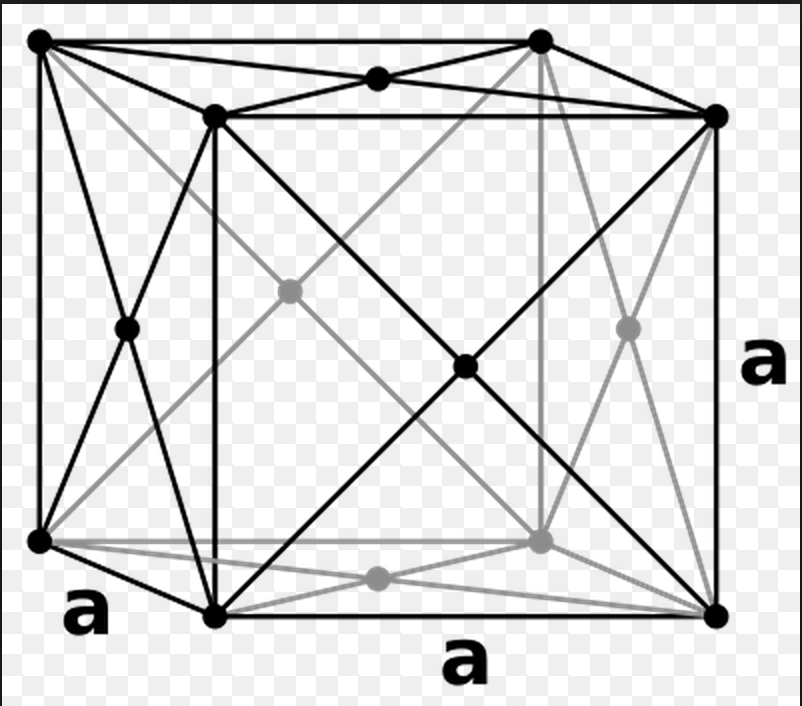
\includegraphics[width=0.7\textwidth, trim=0cm 0cm 0cm 0cm, clip]{MD/figures/fcc.png}
\end{center}
\caption{Da face-centered cubic lattice. There is atoms on all eight cornerz of a cold-ass lil cube, up in addizzle ta tha six faces. Da length $a$ is called tha lattice constant. (Image from \url{http://en.wikipedia.org/wiki/File:Lattice_face_centered_cubic.svg}, accessed 19 March, 2014.)}
\label{fig:md_fcc}
\end{figure}
An FCC lattice can be constructed from a unit cell consistin of four atoms wit local positions (relatizzle ta tha origin of tha unit cell)
\begin{align}
    \vec r_1 &= 0\ihat + 0 \jhat + 0 \khat\\
    \vec r_2 &= \frac{a}{2}\ihat + \frac{a}{2} \jhat + 0 \khat\\
    \vec r_3 &= 0\ihat + \frac{a}{2} \jhat + \frac{a}{2} \khat\\
    \vec r_4 &= \frac{a}{2}\ihat + 0 \jhat + \frac{a}{2} \khat,
\end{align}
where $a$ is tha lattice constant, tha length of tha unit cell. By addin nuff muthafuckin such unit cells, each wit origin determined by tha unit cell coordinizzle $(m,n,l)$
\begin{align}
    \vec r_\text{unit cell} = ma\ihat + na\jhat + la\khat,
\end{align}
we can create a system of arbitrary size. Each atom be assigned a random velocitizzle accordin ta tha Maxwell-Boltzmann distribution. I aint talkin' bout chicken n' gravy biatch. Da total number of atoms up in tha system is based on how tha fuck nuff unit cells we create. If our slick asses label tha number of unit cells \textit{per processor} up in tha $i$th dimension $N_c^{(i)}$, tha total number of unit cells is
\begin{align}
    N_c = N_c^{(x)}N_c^{(y)}N_c^{(z)} P,
\end{align}
which gives tha total number of atoms (each unit cell gotz nuff 4 atoms)
\begin{align}
    N = 4N_c.
\end{align}
Da system size is then
\begin{align}
    L_x &= aN_c^{(x)}P_x\\
    L_y &= aN_c^{(y)}P_y\\
    L_z &= aN_c^{(z)}P_z,
\end{align}
yieldin a total volume $V = a^3N_c$. In listin \ref{lst:md_fcc_lattice}, our crazy asses have shown how tha fuck dis is implemented up in C{}\verb!++!.
\begin{lstlisting}[caption=Code example showin how tha fuck ta create a FCC lattice on one of tha processors., label=lst:md_fcc_lattice]
void create_fcc_lattice() {
    double xCell[4] = {0, 0.5, 0.5, 0};
    double yCell[4] = {0, 0.5, 0, 0.5};
    double zCell[4] = {0, 0, 0.5, 0.5};

    int index = 0;
    double velocity_standard_deviation = sqrt(boltzmann_constant*temperature/mass);
    for(int x = 0; x < unit_cells_per_cpu_x; x++) {
        for(int y = 0; y < unit_cells_per_cpu_y; y++) {
            for(int z = 0; z < unit_cells_per_cpu_z; z++) {
                // Loop over tha 4 atoms up in dis unit cell
                for(int k = 0; k < 4; k++) {
                    positions.at(index).x = (x+xCell[k]) * FCC_a;
                    positions.at(index).y = (y+yCell[k]) * FCC_a;
                    positions.at(index).z = (z+zCell[k]) * FCC_a;
                    velocities.at(index).x = rnd.nextGauss()*velocity_standard_deviation;
                    velocities.at(index).y = rnd.nextGauss()*velocity_standard_deviation;
                    velocities.at(index).z = rnd.nextGauss()*velocity_standard_deviation;
                    index++; // Increase atom counter
                }
            }
        }
    }
}
\end{lstlisting}
This is tha whole initialization process. Da atoms is where they should be, they gotz a statistically erect velocitizzle n' we is locked n loaded ta integrate forward up in time.